\chapter{Felhasználói dokumentáció}
\label{ch:user}

\section{Áttekintés}

Az alkalmazás böngészőben fut. Egy oldalból áll, mely nagy részét egy interaktív térkép foglalja el (\ref{fig:screenshot-welcome}). A képernyő bal oldalán egy vezérlőpanel található, melyen keresztül az alkalmazás irányítható. Az alkalmazás használatához nincs szükség regisztrációra vagy bejelentkezésre.

\begin{figure}[H]
	\centering
	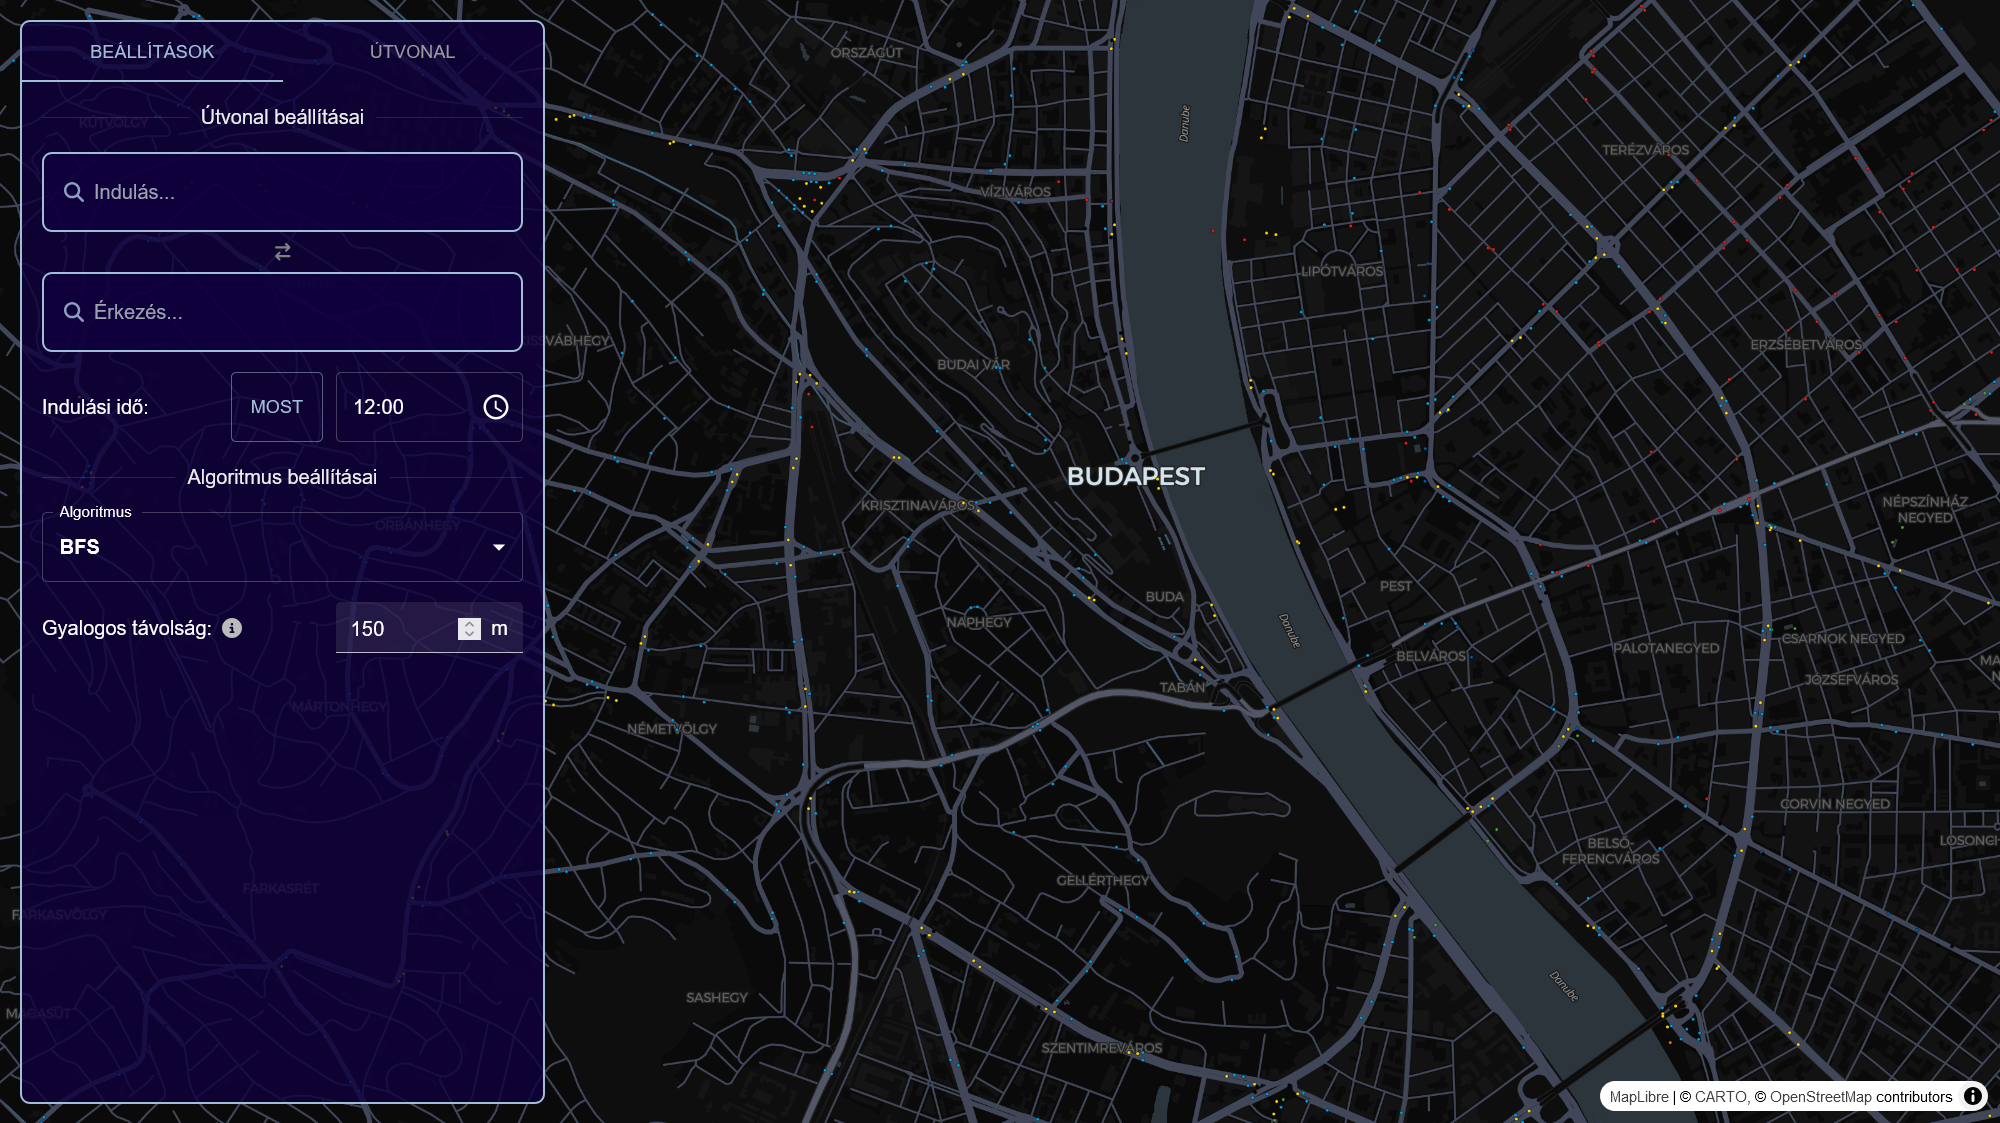
\includegraphics[width=0.8\textwidth,frame]{screenshot_welcome}
	\caption{Az alkalmazás felülete térképpel és vezérlőpanellel}
	\label{fig:screenshot-welcome}
\end{figure}

A térkép navigációja egérrel történik; a térkép nagyítása és kicsinyítése a görgetőkerékkel, a térkép mozgatása pedig az egér bal gombjának lenyomásával és húzásával. A térképen a BKK és a MÁV-HÉV járatainak a megállói láthatók, amik egy-egy színes körrel van jelölve, melyeknek a színét a megállóhoz tartozó járatok színe\footnote{A színek a közlekedési társaságok által használt, közismert színek (pl. a villamosok sárgák, a trolik pirosak).} határozza meg.

\section{Definíciók}

\begin{itemize}
	\item \textbf{Gráf:} Formálisan csúcsok és élek halmaza, ahol minden él két csúcsot köt össze. Az alkalmazás által használt modellben a közlekedési hálózatot egy irányított, súlyozott gráffal modellezzük, így "gráf" alatt a továbbiakban ezt értjük, amennyiben mást nem jelzünk.
	\item \textbf{Csúcs:} A gráf eleme, mely egy megállót jelképez. A továbbiakban a "csúcs" és a "megálló" kifejezések egymás szinonimájaként értendőek, kontextustól függően használjuk őket.
	\item \textbf{Él:} A gráf eleme, mely két csúcsot köt össze. Az élek irányítottak, azaz csak egy irányba utazhatóak; illetve súlyozottak, azaz minden élhez egy súlyt rendelünk, mely az élen való áthaladás költségét jelképezi. Az alkalmazásban két féle él található:
	\begin{compactenum}
		\item \textbf{Utazási él:} Két megálló közötti közvetlen járatot jelképez, melynek a súlya az utazás időtartamának és a járatra való várakozás idejének az összege. Ez utóbbi alól az első utazási él mentesül, hiszen az csak későbbi indulást jelent, nem várakozást.\\\textit{Megjegyzés: A program csak olyan járatokat vesz figyelembe, melyekre a várakozási idő nem haladja meg a 60 percet.}
		\item \textbf{Átszállási él:} Két megálló közötti gyaloglást jelképez, melynek a súlya a $2 \text{perc} + 1 \frac{\text{másodperc}}{\text{méter}}$ képlet alapján számolódik, vagyis minden átszállás alapsúlya 2 perc, és az utak közötti távolság légvonalban.\\\textit{Megjegyzés: Amennyiben az útvonal első éle átszállási él, annak 0 a súlya --- ez azért van, mert könnyű az azonos nevű és egy helyen lévő megállókat összekeverni választáskor, és ezzel a módszerrel akadályozza meg a program azt, hogy egy ilyen hiba miatt hosszabbnak tűnjön az út, mint amilyen valójában.}
	\end{compactenum}
\end{itemize}

\section{Útvonal beállításai}

Útvonal tervezéséhez szükség van egy indulási időpont\footnote{Az indulási idő budapesti időzóna szerint értendő, az alapértelmezett értéke az aktuális helyi idő.}, illetve egy kiinduló- és egy úticél megadására. Célpontoknak a térképen szereplő megállók közül kell választani, egyéb koordináta/cím megadása nem lehetséges. Ezeknek a megadására a vezérlőpanel "BEÁLLÍTÁSOK" fülén van lehetőség (\ref{fig:screenshot-settings-route}).

\begin{figure}[H]
	\centering
	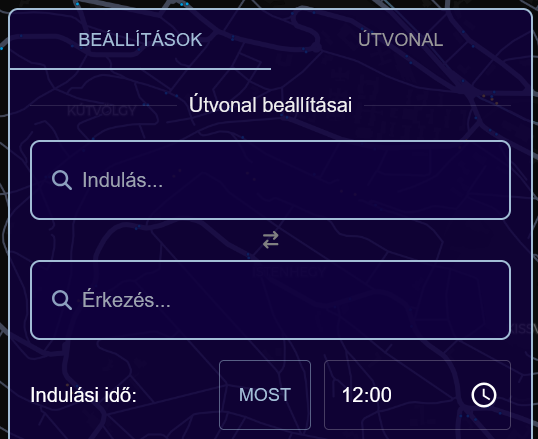
\includegraphics[width=0.5\textwidth,frame]{screenshot_settings_route}
	\caption{Az indulási idő, illetve a kiinduló- és célállomás beállítása}
	\label{fig:screenshot-settings-route}
\end{figure}

Állomások választásához a megfelelő mezőbe kell írni, majd kattintással kiválasztani a megfelelő megállót --- nem elég a nevét beírni, hiszen több, egymástól távoli megálló is rendelkezhet ugyanazzal a névvel (\ref{fig:screenshot-search-stop}). Megfelelő megálló választásához segítségképpen a listában a megállókból induló járatok is megjelennek az adott megálló neve alatt.

A kiinduló- és célállomás felcserélése a két beviteli mező közti dupla nyílra kattintva lehetséges (\ref{fig:screenshot-settings-route}).

\begin{figure}[H]
	\centering
	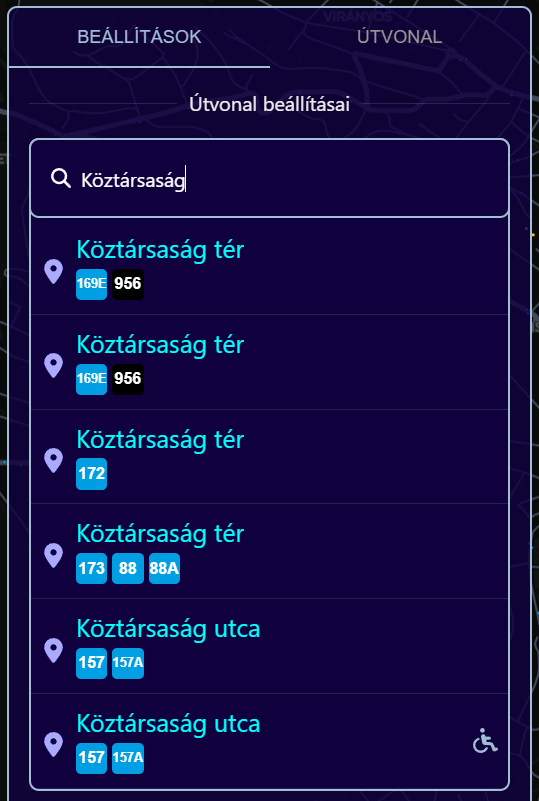
\includegraphics[width=0.4\textwidth,frame]{screenshot_search_stop}
	\caption{Az egyik \emph{Köztársaság tér} nevű megálló Törökbálinton, a másik Pécelen található}
	\label{fig:screenshot-search-stop}
\end{figure}

A térképen az egeret egy megálló fölé helyezve megjelenik annak a neve (\ref{fig:screenshot-tooltip-stop-name}); ez segítséget nyújthat, ha nem ismerjük a célpontunk közelében lévő megállók nevét.

\begin{figure}[H]
	\centering
	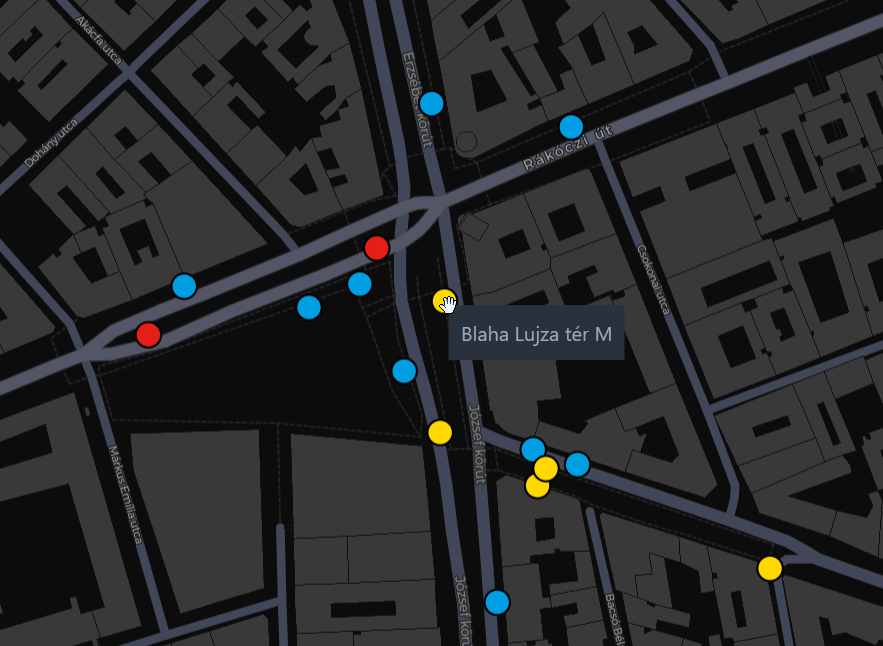
\includegraphics[width=0.8\textwidth,frame]{screenshot_tooltip_stop_name}
	\caption{A kurzor alatt lévő megálló neve egy információs buborékban jelenik meg}
	\label{fig:screenshot-tooltip-stop-name}
\end{figure}

\section{Algoritmus kiválasztása}

\subsection{Választható algoritmusok}

Az útvonalkereséshez négy különböző algoritmus használható, ezekről részletesebben a \ref{ch:TODO implementation}.~fejezetben olvashatunk.

\paragraph{Áttekintés az algoritmusokról:}
\begin{enumerate}
	\item \textbf{BFS}: A "Breadth-First Search", azaz szélességi gráfbejárás egy soralapú algoritmus, ahol az újonnan felfedezett megállók egy sor (FIFO adatszerkezet) végére kerülnek be, így először az 1 megálló távolságra lévő megállók kerülnek felfedezésre, majd a 2, stb. . Az algoritmus alapvetően súlyozatlan gráfokon operál, súlyozott gráfokra való alkalmazásakor is figyelmen kívül hagyja az élek súlyát. Ennek következtében az útkeresés eredményeként garantáltan a legkevesebb megállóból álló utat kapjuk meg, attól függetlenül, hogy az adott út mennyi időbe telik. Ennek az algoritmusnak a futásideje egy hagyományos gráfon a legrosszabb esetben $O(|V| + |E|)$, ahol $V$ a csúcsok, $E$ az élek száma a gráfban.
	\item \textbf{Dijkstra-algoritmus}: Az algoritmus a feltalálójáról, Edsger W. Dijkstra informatikusról kapta a nevét, és egy súlyozott gráfban keresi meg a legkisebb súlyú utat egy kiindulópontból az összes többi csúcsba. Az algoritmus a BFS-sel szemben egy prioritási sort használ, ahol a sor elemei a gráf csúcsai, és súly szerinti sorrendben kerülnek feldolgozásra. (Egy-egy csúcs súlya jelen esetben a kezdőállomásból való utazási távolságnak felel meg.) Az alkalmazásban elérhető algoritmusok közül ez az egyetlen, amely garantálja a legrövidebb utazási időt, viszont futásidőben a prioritási sor manipulálásának a komplexitásának\footnote{Az alkalmazás egy kupaccal implementálja a prioritási sort, így egy elem beillesztésének és eltávolításának a komplexitása legrosszabb esetben egyaránt $O(\log n)$.} következtében az algoritmus komplexitása is magasabb a BFS-hez képest. Az algoritmus futásideje egy hagyományos gráfon a legrosszabb esetben $O((|V| + |E|) \log |V|)$.
	\item \textbf{Mohó algoritmus}: A mohó algoritmus a Dijkstra-algoritmushoz hasonlóan egy prioritásos soron alapul, azonban bevezeti a heurisztika fogalmát. A heurisztika egy olyan függvény, amely egy "megérzést" ad egy adott csúcsról, azaz megbecsüli, hogy az adott csúcs mennyire jó választás lehet a következő lépésben. Ebben az alkalmazásban ennek az implementációja a csúcs távolsága a célállomástól, a Föld felszínén egyenes vonalban utazott méterekben mérve\footnote{A képlet nem ugyan nem veszi figyelembe a tengerszint feletti magasságot, de ez Budapesten és környékén nem tesz drasztikus különbséget, így elfogadjuk közelítésnek.}. Az algoritmus a prioritási sorban a heurisztika értéke szerinti sorrendben dolgozza fel a csúcsokat, így általában sokkal gyorsabban eljut a célállomásba, viszont a BFS-hez hasonlóan ez sem veszi figyelembe az utazási időt, így praktikus használatra általában nem alkalmas. Az algoritmus futásideje egy hagyományos gráfon a legrosszabb esetben $O((|V| + |E|) \log |V|)$.
	\item \textbf{A* algoritmus}: Az A* algoritmus egy továbbfejlesztett mohó algoritmus, amely a Dijkstra-algoritmus és a mohó algoritmus előnyeit igyekszik ötvözni. Az algoritmus a csúcsok súlyát (azaz a kezdőállomástól való utazási időt) és a heurisztikát (a csúcs távolságát a célállomástól) együtt veszi figyelembe a prioritási sorban, így a legjobb választásnak tűnő csúcsokat feldolgozva igyekszik a lehető leggyorsabban eljutni a célállomásba. A* algoritmus választásakor módunk van megadni egy súlyozó faktort, amellyel a heurisztika értékét szorozzuk, így az algoritmus viselkedését befolyásolhatjuk. Alacsonyabb szorzó esetén a Dijkstra-algoritmusra hasonlító viselkedést kapunk (lassabb futásidő, de rövidebb út), magasabb szorzó esetén a mohó algoritmushoz hasnlót (gyorsabb futásidő, de könnyebben eltér a legrövidebb úttól). Az alapértelmezett szorzó $1$, de saját tapasztalataim szerint a $0.3-0.5$ körüli súly jó egyensúlyt biztosít a futásidő és a "használható" eredmény között. Az algoritmus futásideje egy hagyományos gráfon a legrosszabb esetben $O((|V| + |E|) \log |V|)$.
\end{enumerate}

\paragraph{Röviden összefoglalva:}

\begin{compactitem}
	\item \textbf{BFS:} Legkevesebb megállóból álló útvonalat ad, de nem veszi figyelembe az utazási időt.
	\item \textbf{Dijkstra:} Garantáltan a legrövidebb utazási időt adja, de magasabb futásidővel jár.
	\item \textbf{Mohó:} Általában jelentősen gyorsabb a futásideje, de sem az utazási időt, sem az utazott megállók számát nem veszi figyelembe.
	\item \textbf{A*:} Kompromisszum a Dijkstra és a mohó algoritmus között, súlyozó faktorral befolyásolhatjuk a viselkedését.
\end{compactitem}

\subsection{Algoritmusok beállításai}

Az alapértelmezett algoritmus a BFS. Ezt az útvonal beállításai alatt, úgyszintén a vezérlőpanel "BEÁLLÍTÁSOK" fülén lehet megváltoztatni (\ref{fig:screenshot-settings-algorithm}).

\begin{figure}[H]
	\centering
	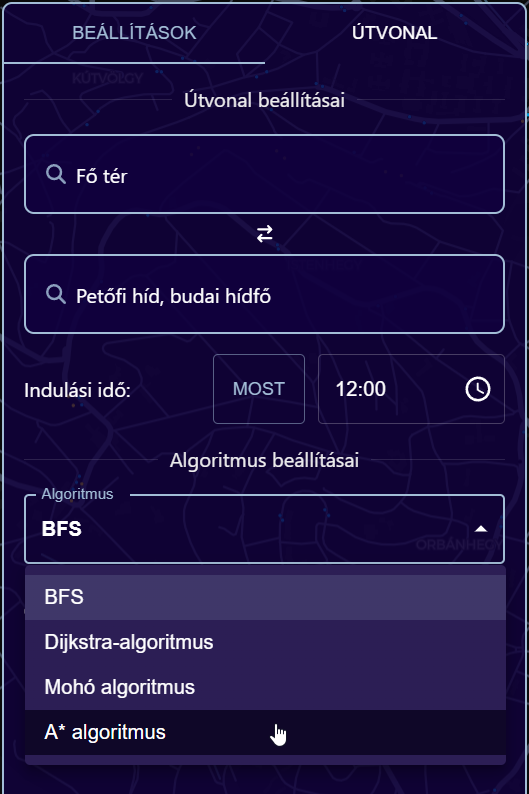
\includegraphics[width=0.5\textwidth,frame]{screenshot_settings_algorithm}
	\caption{Az elérhető algoritmusok listája}
	\label{fig:screenshot-settings-algorithm}
\end{figure}

Választott algoritmustól függetlenül beállítható az is, hogy mi a maximális sétáló távolság, amin belül az alkalmazás felajánl átszállásokat. Ennek az alapértelmezett értéke 150 méter, ami tapasztalataim szerint általában elég azonos nevű, egy csoportban lévő megállók közti átszálláshoz.

Amennyiben a választott algoritmus az A*, akkor a heurisztika súlyozó faktora is beállítható, mely alapértelmezetten $1$ (\ref{fig:screenshot-settings-heuristic}).

\begin{figure}[H]
	\centering
	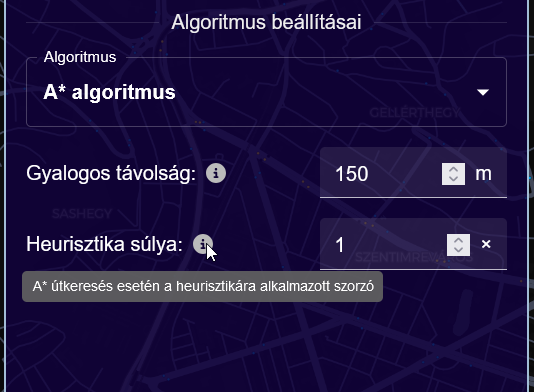
\includegraphics[width=0.7\textwidth,frame]{screenshot_settings_heuristic}
	\caption{A beállításokat információs buborékok magyarázzák}
	\label{fig:screenshot-settings-heuristic}
\end{figure}

\section{Útvonal tervezése}

Amennyiben megtörtént a kezdő- és célállomás megadása, illetve az algoritmust és annak paraméter(ei)t is beállítottuk, megkezdődhet az útvonal tervezése. Ez a vezérlőpanel "ÚTVONAL" fülén történik, mely érvényes beállítások megadása után válik kattinthatóvá (\ref{fig:screenshot-route-initial}).

\begin{figure}[H]
	\centering
	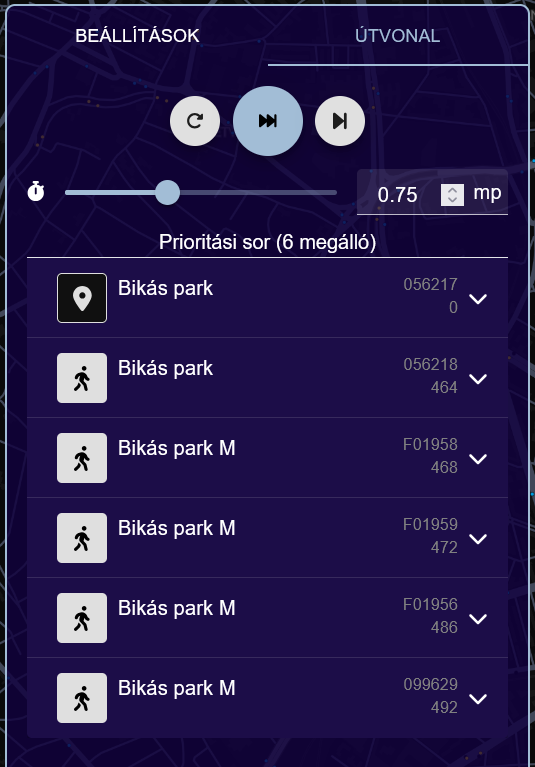
\includegraphics[width=0.4\textwidth,frame]{screenshot_route_initial}
	\caption{Az algoritmus alapállapota az "ÚTVONAL" fülön}
	\label{fig:screenshot-route-initial}
\end{figure}

A fül tetején az algoritmus léptetésére szolgáló gombok találhatók, melyek a következők:
\begin{compactitem}
	\item \textbf{Újraindítás}: Az algoritmus visszaállítása a kezdőállapotba.
	\item \textbf{Futtatás}: Az algoritmus addig fut, amíg el nem éri a célállomást. Amíg az algoritmus fut, a többi gomb nem érhető el, ez pedig átváltozik \textbf{Szüneteltetés} gombbá, ami leállítja az algoritmust.
	\item \textbf{Léptetés}: Az algoritmus egy lépéssel halad előre, majd megáll.
\end{compactitem}

Ezek alatt egy csúszka található, amelyen azt állíthatjuk be, hogy az algoritmus léptetéskor mennyit várakozik két lépés között. Az alapértelmezett értéke $0.75$ másodperc.
\textit{Megjegyzés: Természetesen lehetséges, hogy az alkalmazás többet várakozik a beállítottnál, különösen alacsony értékek esetén. 0 másodperc esetén az algoritmus a lehető leggyorsabban fut.}

\begin{figure}[H]
	\centering
	\subcaptionbox{Vestibulum quis mattis urna}{
		
\includegraphics[width=0.45\linewidth]{elte_cimer_szines}}
	\hspace{5pt}
	\subcaptionbox{Donec hendrerit quis dui sit amet venenatis}{
		
\includegraphics[width=0.45\linewidth]{elte_cimer_szines}}
	\caption{Aenean porttitor mi volutpat massa gravida}
	\label{fig:example-2}
\end{figure}


Lorem ipsum dolor sit amet $\mathbb{N}$\nomenclature{$\mathbb{N}$}{Set of natural numbers}, consectetur adipiscing elit. Duis nibh leo, dapibus in elementum nec, aliquet id sem. Suspendisse potenti. Nullam sit amet consectetur nibh. Donec scelerisque varius turpis at tincidunt. Cras a diam in mauris viverra vehicula. Vivamus mi odio, fermentum vel arcu efficitur, lacinia viverra nibh. Aliquam aliquam ante mi, vel pretium arcu dapibus eu. Nulla finibus ante vel arcu tincidunt, ut consectetur ligula finibus. Mauris mollis lectus sed ipsum bibendum, ac ultrices erat dictum. Suspendisse faucibus euismod lacinia $\mathbb{Z}$\nomenclature{$\mathbb{Z}$}{Set of integer numbers}.


\section{Felsorolások}

Etiam vel odio ante. Etiam pulvinar nibh quis massa auctor congue. Pellentesque quis odio vitae sapien molestie vestibulum sit amet et quam. Pellentesque vel dui eget enim hendrerit finibus at sit amet libero. Quisque sollicitudin ultrices enim, nec porta magna imperdiet vitae. Cras condimentum nunc dui, eget molestie nunc accumsan vel.

\begin{itemize}
	\item Fusce in aliquet neque, in pretium sem.
	\item Donec tincidunt tellus id lectus pretium fringilla.
	\item Nunc faucibus, erat pretium tempus tempor, tortor mi fringilla neque, ac congue ex dui vitae mauris.
\end{itemize}

Donec dapibus sodales ante, at scelerisque nunc laoreet sit amet. Mauris porttitor tincidunt neque, vel ullamcorper neque pulvinar et. Integer eu lorem euismod, faucibus lectus sed, accumsan felis. Nunc ornare mi at augue vulputate, eu venenatis magna mollis. Nunc sed posuere dui, et varius nulla. Sed mollis nibh augue, eget scelerisque eros ornare nec.

\begin{enumerate}
	\item\label{step:first} Donec pretium et quam a cursus. Ut sollicitudin tempus urna et mollis.
	\item Aliquam et aliquam turpis, sed fermentum mauris. Nulla eget ex diam.
	\item Donec eget tellus pharetra, semper neque eget, rutrum diam \ref{step:first}.~lépés.
\end{enumerate}

Praesent porta, metus eget eleifend consequat, eros ligula eleifend ex, a pellentesque mi est vitae urna. Vivamus turpis nunc, iaculis non leo eget, mattis vulputate tellus. Maecenas rutrum eros sem, pharetra interdum nulla porttitor sit amet. In vitae viverra ante. Maecenas sit amet placerat orci, sed tincidunt velit. Vivamus mattis, enim vel suscipit elementum, quam odio venenatis elit\footnote{Phasellus faucibus varius purus, nec tristique enim porta vitae.}, et mollis nulla nunc a risus. Praesent purus magna, tristique sed lacus sit amet, convallis malesuada magna. 

\begin{description}
	\item[Vestibulum venenatis] malesuada enim, ac auctor erat vestibulum et. Phasellus id purus a leo suscipit accumsan.
	\item[Orci varius natoque] penatibus et magnis dis parturient montes, nascetur ridiculus mus. Nullam interdum rhoncus nisl, vel pharetra arcu euismod sagittis. Vestibulum ac turpis auctor, viverra turpis at, tempus tellus.
	\item[Morbi dignissim] erat ut rutrum aliquet. Nulla eu rutrum urna. Integer non urna at mauris scelerisque rutrum sed non turpis.
\end{description}

\subsection{Szoros térközű felsorolások}

Phasellus ultricies, sapien sit amet ultricies placerat, velit purus viverra ligula, id consequat ipsum odio imperdiet enim:
\begin{compactenum}
	\item Maecenas eget lobortis leo.
	\item Donec eget libero enim.
	\item In eu eros a eros lacinia maximus ullamcorper eget augue.
\end{compactenum}

\bigskip

In quis turpis metus. Proin maximus nibh et massa eleifend, a feugiat augue porta. Sed eget est purus. Duis in placerat leo. Donec pharetra eros nec enim convallis:
\begin{compactitem}
	\item Pellentesque odio lacus.
	\item Maximus ut nisl auctor.
	\item Sagittis vulputate lorem.
\end{compactitem}

\bigskip

Vestibulum ante ipsum primis in faucibus orci luctus et ultrices posuere cubilia Curae; Sed lorem libero, dignissim vitae gravida a, ornare vitae est.
\begin{compactdesc}
	\item[Cras maximus] massa commodo pellentesque viverra.
	\item[Morbi sit] amet ante risus. Aliquam nec sollicitudin mauris
	\item[Ut aliquam rhoncus sapien] luctus viverra arcu iaculis posuere
\end{compactdesc}


\section{Képek, ábrák}

Aliquam vehicula luctus mi a pretium. Nulla quam neque, maximus nec velit in, aliquam mollis tortor. Aliquam erat volutpat. Curabitur vitae laoreet turpis. Integer id diam ligula. Nulla sodales purus id mi consequat, eu venenatis odio pharetra. Cras a arcu quam. Suspendisse augue risus, pulvinar a turpis et, commodo aliquet turpis. Nulla aliquam scelerisque mi eget pharetra. Mauris sed posuere elit, ac lobortis metus. Proin lacinia sit amet diam sed auctor. Nam viverra orci id sapien sollicitudin, a aliquam lacus suscipit, \ref{fig:example-1}.~ábra:

\begin{figure}[H]
	\centering
	
\includegraphics[width=0.6\textwidth,height=100px]{elte_cimer_szines}
	\caption{Quisque ac tincidunt leo}
	\label{fig:example-1}
\end{figure}

\subsection{Képek szegélyezése}

Ut aliquet nec neque eget fermentum. Cras volutpat tellus sed placerat elementum. Quisque neque dui, consectetur nec finibus eget, blandit id purus. Nam eget ipsum non nunc placerat interdum.

\begin{figure}[H]
	\centering
	
\includegraphics[width=0.6\textwidth,height=100px,frame]{elte_cimer_szines}
	\caption{Quisque ac tincidunt leo}
\end{figure}

\subsection{Képek csoportosítása}

In non ipsum fermentum urna feugiat rutrum a at odio. Pellentesque habitant morbi tristique senectus et netus et malesuada fames ac turpis egestas. Nulla tincidunt mattis nisl id suscipit. Sed bibendum ac felis sed volutpat. Nam pharetra nisi nec facilisis faucibus. Aenean tristique nec libero non commodo. Nulla egestas laoreet tempus. Nunc eu aliquet nulla, quis vehicula dui. Proin ac risus sodales, gravida nisi vitae, efficitur neque, \ref{fig:example-2}.~ábra:

\begin{figure}[H]
	\centering
	\subcaptionbox{Vestibulum quis mattis urna}{
		
\includegraphics[width=0.45\linewidth]{elte_cimer_szines}}
	\hspace{5pt}
	\subcaptionbox{Donec hendrerit quis dui sit amet venenatis}{
		
\includegraphics[width=0.45\linewidth]{elte_cimer_szines}}
	\caption{Aenean porttitor mi volutpat massa gravida}
	\label{fig:example-2}
\end{figure}

Nam et nunc eget elit tincidunt sollicitudin. Quisque ligula ipsum, tempor vitae tortor ut, commodo rhoncus diam. Pellentesque habitant morbi tristique senectus et netus et malesuada fames ac turpis egestas. Phasellus vehicula quam dui, eu convallis metus porta ac.


\section{Táblázatok}

Nam magna ex, euismod nec interdum sed, sagittis nec leo. Nam blandit massa bibendum mattis tristique. Phasellus tortor ligula, sodales a consectetur vitae, placerat vitae dolor. Aenean consequat in quam ac mollis. 

\begin{table}[H]
	\centering
	\begin{tabular}{ | m{0.25\textwidth} | m{0.65\textwidth} | }
		\hline
		\textbf{Phasellus tortor} & \textbf{Aenean consequat} \\
		\hline \hline
		\emph{Sed malesuada} & Aliquam aliquam velit in convallis ultrices. \\
		\hline
		\emph{Purus sagittis} &  Quisque lobortis eros vitae urna lacinia euismod. \\
		\hline
		\emph{Pellentesque} & Curabitur ac lacus pellentesque, eleifend sem ut, placerat enim. Ut auctor tempor odio ut dapibus. \\
		\hline
	\end{tabular}
	\caption{Maecenas tincidunt non justo quis accumsan}
	\label{tab:example-1}
\end{table}

\subsection{Sorok és oszlopok egyesítése}

Mauris a dapibus lectus. Vestibulum commodo nibh ante, ut maximus magna eleifend vel. Integer vehicula elit non lacus lacinia, vitae porttitor dolor ultrices. Vivamus gravida faucibus efficitur. Ut non erat quis arcu vehicula lacinia. Nulla felis mauris, laoreet sed malesuada in, euismod et lacus. Aenean at finibus ipsum. Pellentesque dignissim elit sit amet lacus congue vulputate.

\begin{table}[htb]
	\centering
	\begin{tabular}{ | c | r | r | r | r | r | r | }
		\hline
		\multirow{2}{*}{\textbf{Quisque}} & \multicolumn{2}{ c | }{\textbf{Suspendisse}} & \multicolumn{2}{ c | }{\textbf{Aliquam}} & \multicolumn{2}{ c | }{\textbf{Vivamus}} \\
		\cline{2-7}
		& Proin & Nunc & Proin & Nunc & Proin & Nunc \\
		\hline \hline		
		Leo & 2,80 MB & 100\% & 232 KB & 8,09\% & 248 KB & 8,64\% \\
		\hline
		Vel & 9,60 MB & 100\% & 564 KB & 5,74\% & 292 KB & 2,97\% \\
		\hline
		Auge & 78,2 MB & 100\% & 52,3 MB & 66,88\% & 3,22 MB & 4,12\% \\
		\hline 
	\end{tabular}
	\caption[Rövid cím a táblázatjegyzékbe]{Vivamus ac arcu fringilla, fermentum neque sed, interdum erat. Mauris bibendum mauris vitae enim mollis, et eleifend turpis aliquet.}
	\label{tab:example-2}
\end{table}

\subsection{Több oldalra átnyúló táblázatok}

Nunc porta placerat leo, sit amet porttitor dui porta molestie. Aliquam at fermentum mi. Maecenas vitae lorem at leo tincidunt volutpat at nec tortor. Vivamus semper lacus eu diam laoreet congue. Vivamus in ipsum risus. Nulla ullamcorper finibus mauris non aliquet. Vivamus elementum rhoncus ex ut porttitor.

\begin{center}
	\begin{longtable}{ | p{0.3\textwidth} | p{0.7\textwidth} | }
		
		\hline
		\multicolumn{2}{|c|}{\textbf{Praesent aliquam mauris enim}}
		\\ \hline
		
		\emph{Suspendisse potenti} & \emph{Lorem ipsum dolor sit amet}
		\\ \hline \hline
		\endfirsthead % első oldal fejléce
		
		\hline
		\emph{Suspendisse potenti} & \emph{Lorem ipsum dolor sit amet}
		\\ \hline \hline
		\endhead % többi oldal fejléce
		
		\hline
		\endfoot % többi oldal lábléce
		
		\endlastfoot % utolsó oldal lábléce
		
		\emph{Praesent}
		& Nulla ultrices et libero sit amet fringilla. Nunc scelerisque ante tempus sapien placerat convallis.
		\\ \hline
		
		\emph{Luctus}
		& Integer hendrerit erat massa, non hendrerit risus convallis at. Curabitur ultrices, justo in imperdiet condimentum, neque tortor luctus enim, luctus posuere massa erat vitae nibh.
		\\ \hline
		
		\emph{Egestas}
		& Duis fermentum feugiat augue in blandit. Mauris a tempor felis. Pellentesque ultricies tristique dignissim. Pellentesque aliquam semper tristique. Nam nec egestas dolor. Vestibulum id elit quis enim fringilla tempor eu a mauris. Aliquam vitae lacus tellus. Phasellus mauris lectus, aliquam id leo eget, auctor dapibus magna. Fusce lacinia felis ac elit luctus luctus.
		\\ \hline
		
		\emph{Dignissim}
		& Praesent aliquam mauris enim, vestibulum posuere massa facilisis in. Suspendisse potenti. Nam quam purus, rutrum eu augue ut, varius vehicula tellus. Fusce dui diam, aliquet sit amet eros at, sollicitudin facilisis quam. Phasellus tempor metus vel augue gravida pretium. Proin aliquam aliquam blandit. Nulla id tempus mi. Fusce in aliquam tortor.
		\\ \hline
		
		\emph{Pellentesque}
		& Donec felis nibh, imperdiet a arcu non, vehicula gravida nibh. Quisque interdum sapien eu massa commodo, ac elementum felis faucibus.
		\\ \hline
		
		\emph{Molestie}
		& Cras ullamcorper tellus et auctor ultricies. Maecenas tincidunt euismod lectus nec venenatis. Suspendisse potenti. Pellentesque pretium nunc ut euismod cursus. Nam venenatis condimentum quam. Curabitur suscipit efficitur aliquet. Interdum et malesuada fames ac ante ipsum primis in faucibus.
		\\ \hline
		
		\emph{Vivamus semper}
		& In purus purus, faucibus eu libero vulputate, tristique sodales nunc. Nulla ut gravida dolor. Fusce vel pellentesque mi, vel efficitur eros. Nunc vitae elit tellus. Sed vestibulum auctor consequat. 
		\\ \hline
		
		\emph{Condimentum}
		& Nulla scelerisque, leo et facilisis pretium, risus enim cursus turpis, eu suscipit ipsum ipsum in mauris. Praesent eget pulvinar ipsum, suscipit interdum nunc. Nam varius massa ut justo ullamcorper sollicitudin. Vivamus facilisis suscipit neque, eu fermentum risus. Ut at mi mauris.
		\\ \hline
		
		\caption{Praesent ullamcorper consequat tellus ut eleifend}
		\label{tab:example-3}		
	\end{longtable}
\end{center}